\documentclass{article}%
\usepackage[T1]{fontenc}%
\usepackage[utf8]{inputenc}%
\usepackage{lmodern}%
\usepackage{textcomp}%
\usepackage{lastpage}%
\usepackage{geometry}%
\geometry{top=1in,bottom=1in,left=1in,right=1in}%
\usepackage{tikz}%
%
\usepackage{booktabs}%
\usepackage{pgfplots}%
\usepgfplotslibrary{fillbetween}%
\pgfplotsset{compat=1.18}%
\usepackage{fancyhdr}%
\usepackage{placeins}%
\usepackage{mathpazo}%
\usepackage{float}%
\pagestyle{fancy}%
\fancyhf{}%
\rhead{\today}%
\lhead{Osdag Structural Analysis - Comprehensive Report}%
\cfoot{\thepage}%
\title{Detailed Engineering Report: Simply Supported Beam Analysis}%
\author{Osdag Internship Project {-} Advanced Module}%
\date{\today}%
%
\begin{document}%
\normalsize%
\maketitle%
\thispagestyle{empty}%
\tableofcontents%
\newpage%
\section{Executive Summary}%
\label{sec:ExecutiveSummary}%
This comprehensive report details the structural response of a simply supported beam. %
The analysis evaluates reactions at supports and internal force distributions (Shear and Moment) based on the specified loading conditions. %
The beam has a total span of 15.00 meters and is subjected to 1 distinct loading elements.%
\par\medskip%
Key findings include:%
\begin{itemize}%
\item%
Total applied downward force: 90.00 kN%
\item%
Maximum Shear Force: 45.00 kN at x = 0.00 m%
\item%
Maximum Bending Moment: 168.75 kNm at x = 7.48 m%
\end{itemize}

%
\section{Methodology}%
\label{sec:Methodology}%
The analysis is performed using the principles of static equilibrium. %
The beam is discretized into 500 segments to ensure high resolution in the resulting diagrams.%
\subsection{Global Equilibrium}%
\label{subsec:GlobalEquilibrium}%
The support reactions \$R\_A\$ and \$R\_B\$ are calculated by taking moments about support A:%
\[ \sum M_A = 0 \implies R_B \cdot L = \sum (P_i \cdot x_i) + \sum (w_j \cdot L_j \cdot x_{centroid,j}) \]%
Once \$R\_B\$ is determined, \$R\_A\$ is found using vertical force balance:%
\[ \sum F_y = 0 \implies R_A = \sum Load_{Total} - R_B \]

%
\subsection{Internal Forces}%
\label{subsec:InternalForces}%
At any section \$x\$, the shear force \$V(x)\$ and bending moment \$M(x)\$ are derived as:%
\[ V(x) = R_A - \int_{0}^{x} w(x) \, dx - \sum P_i |_{x_i < x} \]%
\[ M(x) = R_A \cdot x - \int_{0}^{x} w(x)(x - \xi) \, d\xi - \sum P_i(x - x_i) |_{x_i < x} \]

%
\section{Input Data}%
\label{sec:InputData}%
The loading data extracted from the Excel file is shown below.%
\subsection{Load Table}%
\label{subsec:LoadTable}%
\begin{table}[H]%
\centering%
\begin{tabular}{lrrrr}
\toprule
Load Type & Magnitude (kN) & Position (m) & Start Position (m) & End Position (m) \\
\midrule
UDL & 6 & NaN & 0 & 15 \\
\bottomrule
\end{tabular}
%
\caption{Load Configuration}%
\end{table}

%
\FloatBarrier%
\section{Analysis \& Visualizations}%
\label{sec:AnalysisVisualizations}%
The structural analysis yielded the following support reactions:\newline%
%
\begin{description}%
\item[$R_A$ (Left Support):]%
 45.00 kN%
\item[$R_B$ (Right Support):]%
 45.00 kN%
\end{description}%
\subsection{Shear Force Diagram (SFD)}%
\label{subsec:ShearForceDiagram(SFD)}%
The maximum absolute shear force is 45.00 kN, occurring at 0.00 m.%


\begin{figure}[H]%
\centering%
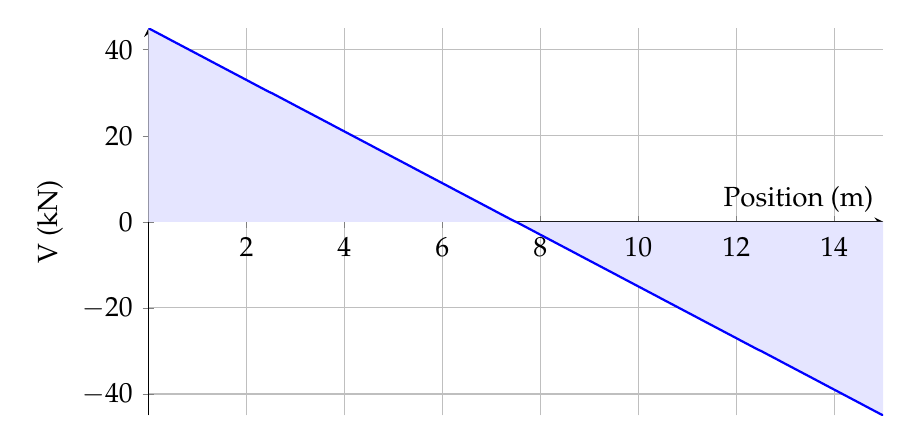
\begin{tikzpicture}%
\begin{axis}[width=0.9\textwidth, height=6.5cm, axis x line=middle, axis y line=left, xlabel={Position (m)}, ylabel={V (kN)}, grid=major, enlarge x limits=false]%
\addplot[name path=f, blue, thick] coordinates {(0.00,45.00) (0.06,44.64) (0.12,44.28) (0.18,43.92) (0.24,43.56) (0.30,43.20) (0.36,42.84) (0.42,42.47) (0.48,42.11) (0.54,41.75) (0.60,41.39) (0.66,41.03) (0.72,40.67) (0.78,40.31) (0.84,39.95) (0.90,39.59) (0.96,39.23) (1.02,38.87) (1.08,38.51) (1.14,38.15) (1.20,37.79) (1.26,37.42) (1.32,37.06) (1.38,36.70) (1.44,36.34) (1.50,35.98) (1.56,35.62) (1.62,35.26) (1.68,34.90) (1.74,34.54) (1.80,34.18) (1.86,33.82) (1.92,33.46) (1.98,33.10) (2.04,32.74) (2.10,32.37) (2.16,32.01) (2.22,31.65) (2.28,31.29) (2.34,30.93) (2.40,30.57) (2.46,30.21) (2.53,29.85) (2.59,29.49) (2.65,29.13) (2.71,28.77) (2.77,28.41) (2.83,28.05) (2.89,27.69) (2.95,27.32) (3.01,26.96) (3.07,26.60) (3.13,26.24) (3.19,25.88) (3.25,25.52) (3.31,25.16) (3.37,24.80) (3.43,24.44) (3.49,24.08) (3.55,23.72) (3.61,23.36) (3.67,23.00) (3.73,22.64) (3.79,22.27) (3.85,21.91) (3.91,21.55) (3.97,21.19) (4.03,20.83) (4.09,20.47) (4.15,20.11) (4.21,19.75) (4.27,19.39) (4.33,19.03) (4.39,18.67) (4.45,18.31) (4.51,17.95) (4.57,17.59) (4.63,17.22) (4.69,16.86) (4.75,16.50) (4.81,16.14) (4.87,15.78) (4.93,15.42) (4.99,15.06) (5.05,14.70) (5.11,14.34) (5.17,13.98) (5.23,13.62) (5.29,13.26) (5.35,12.90) (5.41,12.54) (5.47,12.17) (5.53,11.81) (5.59,11.45) (5.65,11.09) (5.71,10.73) (5.77,10.37) (5.83,10.01) (5.89,9.65) (5.95,9.29) (6.01,8.93) (6.07,8.57) (6.13,8.21) (6.19,7.85) (6.25,7.48) (6.31,7.12) (6.37,6.76) (6.43,6.40) (6.49,6.04) (6.55,5.68) (6.61,5.32) (6.67,4.96) (6.73,4.60) (6.79,4.24) (6.85,3.88) (6.91,3.52) (6.97,3.16) (7.03,2.80) (7.09,2.43) (7.15,2.07) (7.21,1.71) (7.27,1.35) (7.33,0.99) (7.39,0.63) (7.45,0.27) (7.52,-0.09) (7.58,-0.45) (7.64,-0.81) (7.70,-1.17) (7.76,-1.53) (7.82,-1.89) (7.88,-2.25) (7.94,-2.62) (8.00,-2.98) (8.06,-3.34) (8.12,-3.70) (8.18,-4.06) (8.24,-4.42) (8.30,-4.78) (8.36,-5.14) (8.42,-5.50) (8.48,-5.86) (8.54,-6.22) (8.60,-6.58) (8.66,-6.94) (8.72,-7.30) (8.78,-7.67) (8.84,-8.03) (8.90,-8.39) (8.96,-8.75) (9.02,-9.11) (9.08,-9.47) (9.14,-9.83) (9.20,-10.19) (9.26,-10.55) (9.32,-10.91) (9.38,-11.27) (9.44,-11.63) (9.50,-11.99) (9.56,-12.35) (9.62,-12.72) (9.68,-13.08) (9.74,-13.44) (9.80,-13.80) (9.86,-14.16) (9.92,-14.52) (9.98,-14.88) (10.04,-15.24) (10.10,-15.60) (10.16,-15.96) (10.22,-16.32) (10.28,-16.68) (10.34,-17.04) (10.40,-17.40) (10.46,-17.77) (10.52,-18.13) (10.58,-18.49) (10.64,-18.85) (10.70,-19.21) (10.76,-19.57) (10.82,-19.93) (10.88,-20.29) (10.94,-20.65) (11.00,-21.01) (11.06,-21.37) (11.12,-21.73) (11.18,-22.09) (11.24,-22.45) (11.30,-22.82) (11.36,-23.18) (11.42,-23.54) (11.48,-23.90) (11.54,-24.26) (11.60,-24.62) (11.66,-24.98) (11.72,-25.34) (11.78,-25.70) (11.84,-26.06) (11.90,-26.42) (11.96,-26.78) (12.02,-27.14) (12.08,-27.51) (12.14,-27.87) (12.20,-28.23) (12.26,-28.59) (12.32,-28.95) (12.38,-29.31) (12.44,-29.67) (12.51,-30.03) (12.57,-30.39) (12.63,-30.75) (12.69,-31.11) (12.75,-31.47) (12.81,-31.83) (12.87,-32.19) (12.93,-32.56) (12.99,-32.92) (13.05,-33.28) (13.11,-33.64) (13.17,-34.00) (13.23,-34.36) (13.29,-34.72) (13.35,-35.08) (13.41,-35.44) (13.47,-35.80) (13.53,-36.16) (13.59,-36.52) (13.65,-36.88) (13.71,-37.24) (13.77,-37.61) (13.83,-37.97) (13.89,-38.33) (13.95,-38.69) (14.01,-39.05) (14.07,-39.41) (14.13,-39.77) (14.19,-40.13) (14.25,-40.49) (14.31,-40.85) (14.37,-41.21) (14.43,-41.57) (14.49,-41.93) (14.55,-42.29) (14.61,-42.66) (14.67,-43.02) (14.73,-43.38) (14.79,-43.74) (14.85,-44.10) (14.91,-44.46) (14.97,-44.82) (15.00,-45.00)};%
\path[name path=axis] (axis cs:0,0) -- (axis cs:15.0,0);%
\addplot[blue!10] fill between[of=f and axis];%
\end{axis}%
\end{tikzpicture}%
\caption{Shear Force Diagram (SFD)}%
\end{figure}

%
\subsection{Bending Moment Diagram (BMD)}%
\label{subsec:BendingMomentDiagram(BMD)}%
The maximum absolute bending moment (critical section) is 168.75 kNm, occurring at 7.48 m.%


\begin{figure}[H]%
\centering%
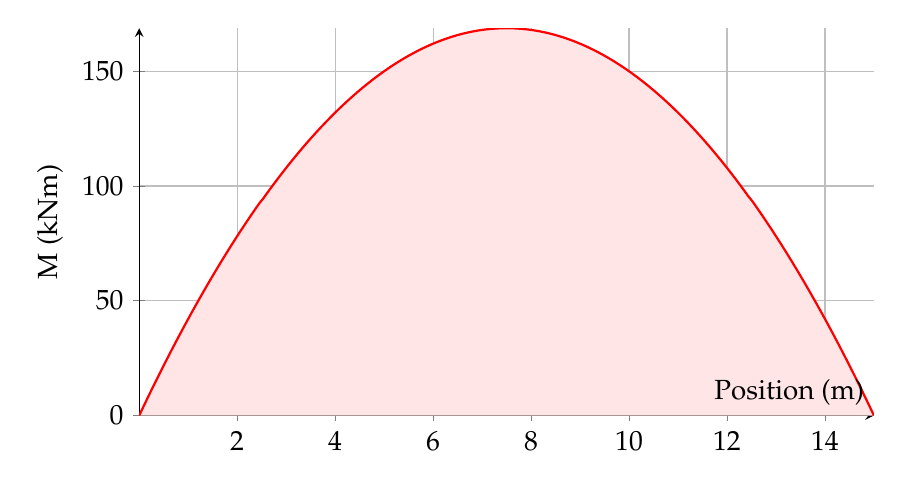
\begin{tikzpicture}%
\begin{axis}[width=0.9\textwidth, height=6.5cm, axis x line=middle, axis y line=left, xlabel={Position (m)}, ylabel={M (kNm)}, grid=major, enlarge x limits=false]%
\addplot[name path=f, red, thick] coordinates {(0.00,0.00) (0.06,2.69) (0.12,5.37) (0.18,8.02) (0.24,10.65) (0.30,13.26) (0.36,15.84) (0.42,18.41) (0.48,20.95) (0.54,23.47) (0.60,25.97) (0.66,28.45) (0.72,30.90) (0.78,33.34) (0.84,35.75) (0.90,38.14) (0.96,40.51) (1.02,42.86) (1.08,45.18) (1.14,47.49) (1.20,49.77) (1.26,52.03) (1.32,54.27) (1.38,56.49) (1.44,58.68) (1.50,60.86) (1.56,63.01) (1.62,65.14) (1.68,67.25) (1.74,69.34) (1.80,71.40) (1.86,73.45) (1.92,75.47) (1.98,77.47) (2.04,79.45) (2.10,81.41) (2.16,83.34) (2.22,85.26) (2.28,87.15) (2.34,89.02) (2.40,90.87) (2.46,92.69) (2.53,94.50) (2.59,96.28) (2.65,98.05) (2.71,99.79) (2.77,101.50) (2.83,103.20) (2.89,104.88) (2.95,106.53) (3.01,108.16) (3.07,109.77) (3.13,111.36) (3.19,112.93) (3.25,114.47) (3.31,116.00) (3.37,117.50) (3.43,118.98) (3.49,120.44) (3.55,121.87) (3.61,123.29) (3.67,124.68) (3.73,126.05) (3.79,127.40) (3.85,128.73) (3.91,130.04) (3.97,131.32) (4.03,132.59) (4.09,133.83) (4.15,135.05) (4.21,136.25) (4.27,137.42) (4.33,138.58) (4.39,139.71) (4.45,140.82) (4.51,141.91) (4.57,142.98) (4.63,144.03) (4.69,145.05) (4.75,146.05) (4.81,147.04) (4.87,148.00) (4.93,148.93) (4.99,149.85) (5.05,150.74) (5.11,151.62) (5.17,152.47) (5.23,153.30) (5.29,154.11) (5.35,154.89) (5.41,155.66) (5.47,156.40) (5.53,157.12) (5.59,157.82) (5.65,158.50) (5.71,159.15) (5.77,159.79) (5.83,160.40) (5.89,160.99) (5.95,161.56) (6.01,162.11) (6.07,162.63) (6.13,163.14) (6.19,163.62) (6.25,164.08) (6.31,164.52) (6.37,164.94) (6.43,165.33) (6.49,165.71) (6.55,166.06) (6.61,166.39) (6.67,166.70) (6.73,166.99) (6.79,167.25) (6.85,167.50) (6.91,167.72) (6.97,167.92) (7.03,168.10) (7.09,168.26) (7.15,168.39) (7.21,168.51) (7.27,168.60) (7.33,168.67) (7.39,168.72) (7.45,168.74) (7.52,168.75) (7.58,168.73) (7.64,168.70) (7.70,168.64) (7.76,168.55) (7.82,168.45) (7.88,168.33) (7.94,168.18) (8.00,168.01) (8.06,167.82) (8.12,167.61) (8.18,167.38) (8.24,167.12) (8.30,166.85) (8.36,166.55) (8.42,166.23) (8.48,165.89) (8.54,165.52) (8.60,165.14) (8.66,164.73) (8.72,164.30) (8.78,163.85) (8.84,163.38) (8.90,162.89) (8.96,162.37) (9.02,161.84) (9.08,161.28) (9.14,160.70) (9.20,160.10) (9.26,159.47) (9.32,158.83) (9.38,158.16) (9.44,157.47) (9.50,156.76) (9.56,156.03) (9.62,155.28) (9.68,154.50) (9.74,153.70) (9.80,152.89) (9.86,152.05) (9.92,151.18) (9.98,150.30) (10.04,149.39) (10.10,148.47) (10.16,147.52) (10.22,146.55) (10.28,145.56) (10.34,144.54) (10.40,143.51) (10.46,142.45) (10.52,141.37) (10.58,140.27) (10.64,139.15) (10.70,138.00) (10.76,136.84) (10.82,135.65) (10.88,134.44) (10.94,133.21) (11.00,131.96) (11.06,130.68) (11.12,129.39) (11.18,128.07) (11.24,126.73) (11.30,125.37) (11.36,123.99) (11.42,122.58) (11.48,121.16) (11.54,119.71) (11.60,118.24) (11.66,116.75) (11.72,115.24) (11.78,113.70) (11.84,112.15) (11.90,110.57) (11.96,108.97) (12.02,107.35) (12.08,105.71) (12.14,104.04) (12.20,102.36) (12.26,100.65) (12.32,98.92) (12.38,97.17) (12.44,95.39) (12.51,93.60) (12.57,91.78) (12.63,89.95) (12.69,88.09) (12.75,86.20) (12.81,84.30) (12.87,82.38) (12.93,80.43) (12.99,78.46) (13.05,76.47) (13.11,74.46) (13.17,72.43) (13.23,70.37) (13.29,68.30) (13.35,66.20) (13.41,64.08) (13.47,61.94) (13.53,59.77) (13.59,57.59) (13.65,55.38) (13.71,53.15) (13.77,50.90) (13.83,48.63) (13.89,46.34) (13.95,44.02) (14.01,41.69) (14.07,39.33) (14.13,36.95) (14.19,34.55) (14.25,32.12) (14.31,29.68) (14.37,27.21) (14.43,24.72) (14.49,22.21) (14.55,19.68) (14.61,17.13) (14.67,14.55) (14.73,11.95) (14.79,9.34) (14.85,6.70) (14.91,4.03) (14.97,1.35) (15.00,0.00)};%
\path[name path=axis] (axis cs:0,0) -- (axis cs:15.0,0);%
\addplot[red!10] fill between[of=f and axis];%
\end{axis}%
\end{tikzpicture}%
\caption{Bending Moment Diagram (BMD)}%
\end{figure}

%
\section{Conclusion}%
\label{sec:Conclusion}%
The analysis of the simply supported beam has been successfully completed. %
The resulting SFD and BMD provide the necessary internal force distributions for further structural design, such as reinforcement calculation or section selection. %
Special attention should be given to the section at x = 7.48 m, where the bending moment is maximized.%
\par\vfill%
\begin{center} \textit{End of Engineering Report} \end{center}

%
\end{document}